This chapter presents the design of a safe controller for the  robotic patient manipulator in 3D Cartesian space, where the unsafe region is defined as an ellipsoid with static boundaries, i.e. fixed in space with respect to time. The unsafe region is defined such that it is within the reach of the instrument tip. 

The robotic patient manipulator constitutes four "arms" (see \autoref{fig:master-slave_surgery}) each comprising a number of arm links, whose joints are fixed by electromagnets that are manually released for positioning of these links; followed by the robot "hand" and instrument links, whose joints are available for automated control on the modified AAU da Vinci robot. Only the controllable part of the robotic patient manipulator, as displayed in \autoref{fig:robot_hand_3d}, is considered in the design of the 3D Cartesian space controller. 

\begin{figure}[htbp]
\centering
\subbottom[Robotic patient manipulator.]{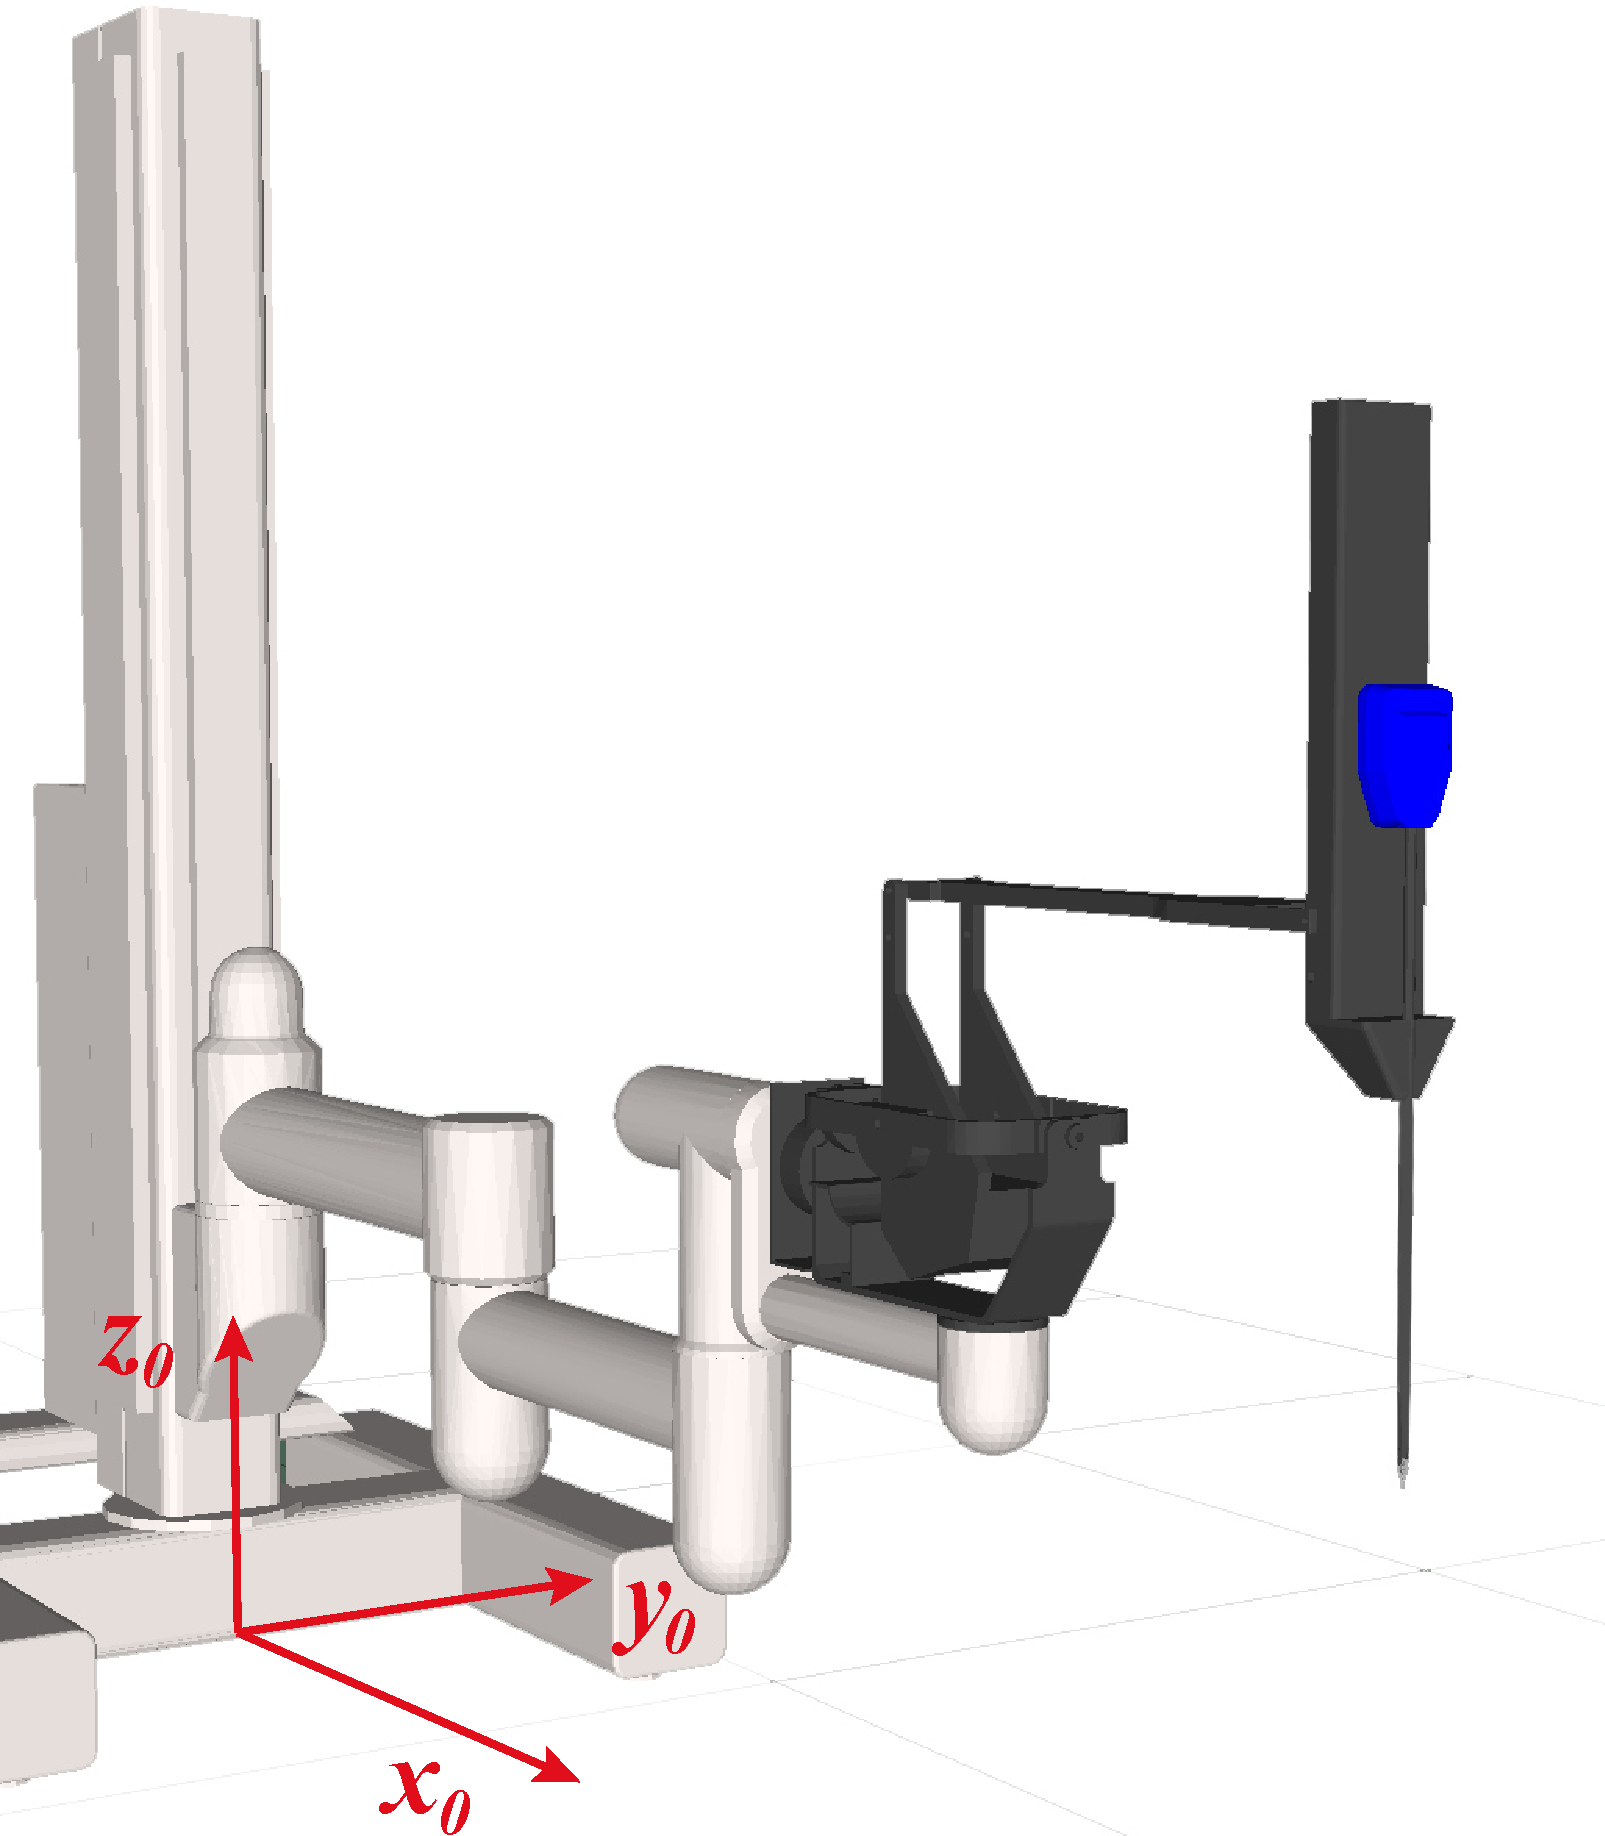
\includegraphics[width=0.45\textwidth]{rviz_09_17_18_frame1.pdf}\label{fig:rviz_09_17_18_frame}}%
	\hspace*{5mm}
\subbottom[Robotic "hand" and instrument.]{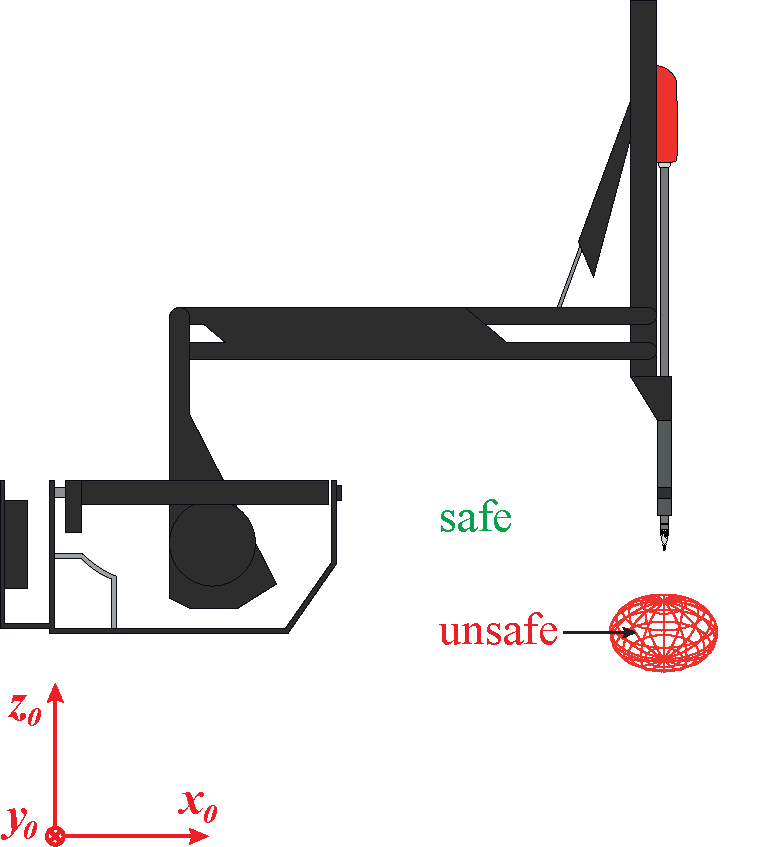
\includegraphics[width=0.45\textwidth]{robot_hand_unsafe_region.pdf}\label{fig:robot_hand_unsafe_region}}%
\caption{Patient manipulator and a fixed region within the reachable space $\mathcal{X}$ that is unsafe, $\mathcal{X}_u$, marked by a red ellipsoid.}
\label{fig:robot_hand_3d}
\end{figure}

The controller is designed for and tested on the da Vinci robot comprising the prismatic slide joint as described in \autoref{chap:cbf_1d_static} as well as five independent revolute joints. In order to design a controller in 3D Cartesian space for the robot, a kinematic description of the robot links and joints is necessary as a translation between the 3D Cartesian space and the 6D joint space.
Hence, before modelling the system and designing a controller, the kinematics of the AAU da Vinci robot is presented in the following section along with considerations for the definition of the coordinate frames and the transformation between them constituting the kinematic description of the robot.


\section{Kinematics of the AAU da Vinci Robot}
A kinematic description of an object requires defining a right-handed coordinate frame fixed in the object and a coordinate frame fixed in inertial space, the latter which the position and orientation of the object can be described relative to. This relative orientation and position of an object (or the frame $i$ fixed in it) with respect to another frame $j=i-1$ can be described through a transformation matrix $T$, containing the orthonormal rotation matrix $R$ and the translation vector $p$ of the frame origin, as 
\begin{equation}
^j_iT = 
\begin{bmatrix}
^j_iR & ^j_ip\\
0 & 1
\end{bmatrix}, \qquad
^j_iT^{-1} = 
\begin{bmatrix}
^j_iR^T & -^j_iR^T\,\,^j_ip\\
0 & 1
\end{bmatrix},
\qquad \text{where} \qquad
^j_ip = 
\begin{bmatrix}
a\\b\\d
\end{bmatrix}
\end{equation}
and the simplest rotation matrices $R$ are rotations about a single axis, which can be combined to obtain an arbitrary rotation
\begin{small}
	\begin{equation}
	R_x(\alpha) = 
	\begin{bmatrix}
	1 & 0 & 0\\
	0 & \cos\alpha & -\sin\alpha\\
	0 & \sin\alpha & \cos\alpha
	\end{bmatrix} 
	\qquad
	R_y(\beta) = 
	\begin{bmatrix}
	\cos\beta & 0 & \sin\beta \\
	0 & 1 & 0\\
	-\sin\beta & 0 & \cos\beta
	\end{bmatrix}
	\qquad
	R_z(\theta) = 
	\begin{bmatrix}
	\cos\theta & -\sin\theta & 0\\
	\sin\theta & \cos\theta & 0\\
	0 & 0 & 1
	\end{bmatrix}
	\label{eq:RxRyRz_chapter}
	\end{equation}
\end{small}

For the robotic patient manipulator comprising a number of links, coordinate frames are defined for each degree of freedom, i.e. placed in each joint such that one of the frame axes is the axis of free rotation or translation. The kinematic chain is now the sequence of alternate links and joints starting from the link fixed in inertial space and ending at the tip of the robotic tool. The link preceding a joint is its parent link, while the link succeeding it is its child link. The transformation between any two frames is given as the product of the transformation matrices in the kinematic chain between them. An example of a sequence of transformations can be seen in \autoref{app:kinematic_model_robot}.

For the resolution of frame definitions it is desired to adapt the  robot coordinate frame convention \gls{dh}, where free rotation/translation always takes place around/along the local $z$ axis. The \gls{dh} convention is preferred because it describes transformations between two successive frames in the kinematic chain on a succinct and standard form 
\begin{equation}
\hspace*{-2mm}
\small
^{i-1}_{\phantom{-1}i} T =
\begin{bmatrix}
R_z(\theta_i) & \begin{bmatrix}0\\ 0\\ d_i\end{bmatrix}\\
0 & 1
\end{bmatrix}
\begin{bmatrix}
R_x(\alpha_i) & \begin{bmatrix}a_i\\ 0\\ 0\end{bmatrix}\\
0 & 1
\end{bmatrix}
\label{eq:dh}
\end{equation}
In the \gls{dh} convention each frame is fixed with respect to its parent link, and its $z$-axis is aligned with the actuation axis of its child link. As seen from \autoref{eq:dh} the free rotation/translation about/along the $z$-axis is implemented (intrinsically) before the fixed rotation/translation about/along the (new) $x$-axis. For more details on the \gls{dh} convention and robot frames defined according to is, see \autoref{sec:denavit_hartenberg}.

%\begin{itemize}
%	\itemsep-1.3mm 
%	\item variable/parameter $\theta_i$ is the angle from $x_{i-1}$ to $x_i$ about $z_{i-1}$
%	\item variable/parameter $d_i$ is the distance from origin $i-1$ to $x_i$ measured along $z_{i-1}$
%	\item parameter $a_i$ is the distance from $z_{i-1}$ to $z_i$ measured along $x_i$
%	\item parameter $\alpha_i$ is the angle from $z_{i-1}$ to $z_i$ about $x_i$
%\end{itemize}

In the robot description in \gls{ros}, however, the kinematics are described in the \texttt{xacro} on the form
\begin{equation}
\hspace*{-2mm}
\small
^{i-1}_{\phantom{-1}i}T =
\begin{bmatrix}
R_z(\text{yaw})R_y(\text{pitch})R_x(\text{roll}) & \begin{bmatrix}a_i\\ b_i\\ d_i\end{bmatrix}\\
0 & 1
\end{bmatrix}
\begin{bmatrix}
R_z(\theta_i^*) & \begin{bmatrix}0\\ 0\\ d_i^* \end{bmatrix}\\
0 & 1
\end{bmatrix}
\label{eq:xacro_transformation_chapter}
\end{equation}
Here fixed translations are implemented first, then RPY rotations (extrinsic roll (about $x$-axis), pitch (about $y$-axis), yaw (about $z$-axis) rotation). Furthermore, the convention here is that each frame (joint) is fixed in its child link (corresponding to the fixed rotations preceding the free rotation), and not in its parent link as in the DH convention. The transformation  $^{i-1}_{\phantom{-1}i} T$ is implemented in joint $i$ in the \texttt{xacro} file  as (for joint 8)
\begin{lstlisting}[language=xml]
<joint name="p4_hand_pitch"  type="revolute">
<origin
xyz="0 0 0"
rpy="1.5708 0 0" />
<parent link="rcm_vitual0" />
<child link="rcm_vitual1" />
<axis xyz="0 0 1" />
...
</joint>
\end{lstlisting}

A compromise is made, defining a new set of frames for the da Vinci kinematics, adhering to the \gls{dh} constraint that each free rotation/translation is about/along the local $z$-axis. The new kinematic frames are visualized in \autoref{fig:p4_hand_compromise_frames_chapter}, the parameters listed in table \ref{tab:new_kin_short}. Furthermore, for simplification of the inverse kinematics solver, the two passive joints mimicking the hand pitch movement are removed from the existing kinematic chain, visualized in \autoref{fig:p4_hand_xacro_frames_chapter}, and parameters listed in table \ref{tab:old_kin_short} for comparison.  



\begin{table}[htbp]
	\small
	\centering
\subbottom[Old robot hand kinematics including mimicking joints, corresponding to \autoref{fig:p4_hand_xacro_frames_chapter}.]{%
	\begin{tabular}{r | rrr | ccc | c l}\hline
		& \multicolumn{3}{c|}{fixed translation  [m]} & \multicolumn{3}{c|}{fixed rotation [rad]} & freedom & \\
		frame  & $a$ ($x$)  & $b$ ($y$)  & $d$ ($z$)  & roll  & pitch & yaw & $\alpha^*, \beta^*, \theta^*$ or $d^*$ & joint name\\\hline
		7 & -0.042 & 0 & 0.161 & 0 & 0 & 0 & $\phantom{-}\alpha_7^*$ & \texttt{hand\_roll} \\
		8 & 0 & 0 & 0 & 0 & -0.288 & 0 & $-\beta_8^*$ & \texttt{hand\_pitch} \\
		9 & 0.011 & 0 & 0.186 & $\pi$ & 0.288 & 0 & $\phantom{-}\beta_8$ & mimic \texttt{hand\_pitch} \\
		10 & 0.520 & 0 & 0 & $\pi$ & 0& 0 &  $-\beta_8$ & mimic \texttt{hand\_pitch} \\
		11 & 0 & 0 & -0.120  & 0 & 0 & 0 & $\phantom{-}d_{11}^*$ & \texttt{instrument\_slide} \\
		12 & 0.052 & 0 & 0 & $\pi$ & 0 & $\pi/2$ & $\phantom{-}\theta_{12}^*$ & \texttt{instrument\_roll} \\
		13 & 0 & 0 & 0.177 & 0 & 0 & 0 & $-\alpha_{13}^*$ & \texttt{instrument\_pitch} \\
		14L & 0 & 0 & 0.009 & $\pi/2$ & $\pi/2$ & 0 & $-\theta_{14L}^*$ & \texttt{instrument\_jaw\_left} \\
		14R & 0 & 0 & 0.009 & $\pi/2$ & $\pi/2$ & 0 & $\phantom{-}\theta_{14R}^*$ & \texttt{instrument\_jaw\_right} \\
	\end{tabular}\label{tab:old_kin_short}}
	\vspace*{1mm}
\subbottom[New robot hand kinematics excluding mimicking joints, corresponding to \autoref{fig:p4_hand_compromise_frames_chapter}.]{%
	\begin{tabular}{r | rrr | ccc | c l}\hline
		& \multicolumn{3}{c|}{fixed translation  [m]} & \multicolumn{3}{c|}{fixed rotation [rad]} & freedom & \\
		frame  & $a$ ($x$)  & $b$ ($y$)  & $d$ ($z$)  & roll  & pitch & yaw & $\theta^*$ or $d^*$ & joint name\\\hline
		7 & 0.482 & 0 & 0.047 & 0 & $\pi/2$ & 0 & $\theta_7^*$ & \texttt{hand\_roll} \\
		8 & 0 & 0 & 0 & $\pi/2$ & 0 & 0 & $\theta_8^*$ & \texttt{hand\_pitch} \\
		9 & 0.097 & 0 & 0 & 0 & $-\pi/2$ &  0 & $d_9^*$ & \texttt{instrument\_slide} \\
		10 & 0 & 0 & 0 & 0 & 0 & 0 & $\theta_{10}^*$ & \texttt{instrument\_roll} \\
		11 & 0 & 0 & 0 & 0 & $\pi/2$ & 0 & $\theta_{11}^*$ & \texttt{instrument\_pitch} \\
		12L & 0.009 & 0 & 0 & $-\pi/2$ & 0 & 0 & $\theta_{12L}^*$ & \texttt{instrument\_jaw\_left} \\
		12R & 0.009 & 0 & 0 & $-\pi/2$ & 0 & 0 & $\theta_{12R}^*$ & \texttt{instrument\_jaw\_right} \\
		\end{tabular}\label{tab:new_kin_short}}
	\caption{Parameters and variables (marked with $^*$) for the robot kinematic description implemented in \gls{ros} and visualized in \autoref{fig:robot_hand_kinematics}.}
	\label{tab:xacro_param_short}
\end{table}

\begin{figure}[htbp]
	\centering
	\subbottom[Old robot hand kinematics including mimick joints, parameters given in table \ref{tab:old_kin_short}.]{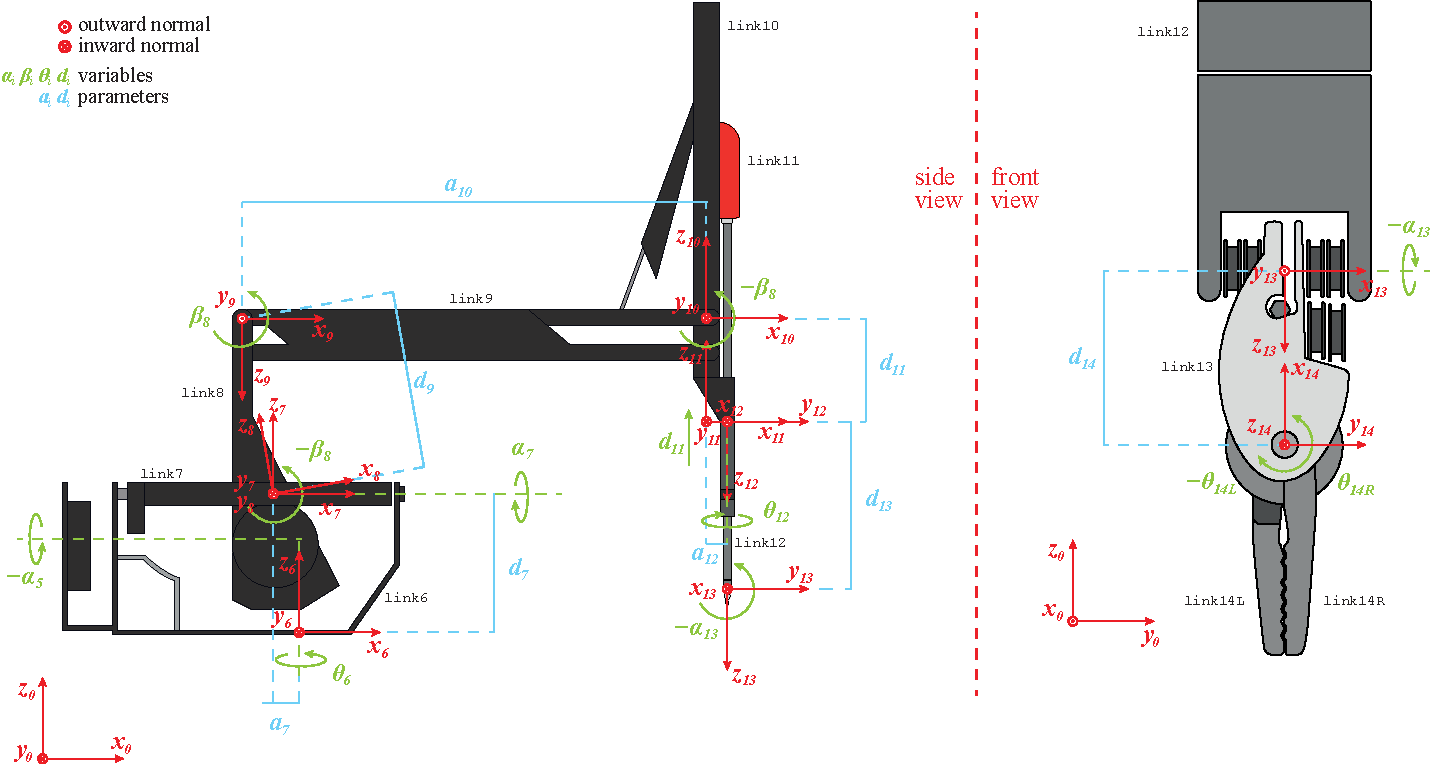
\includegraphics[width=1.15\textwidth]{p4_hand_xacro_frames_chapter.pdf}\label{fig:p4_hand_xacro_frames_chapter}}%
	\vspace*{5mm}
	\subbottom[New robot hand kinematics excluding mimick joints, parameters given in table \ref{tab:new_kin_short}.]{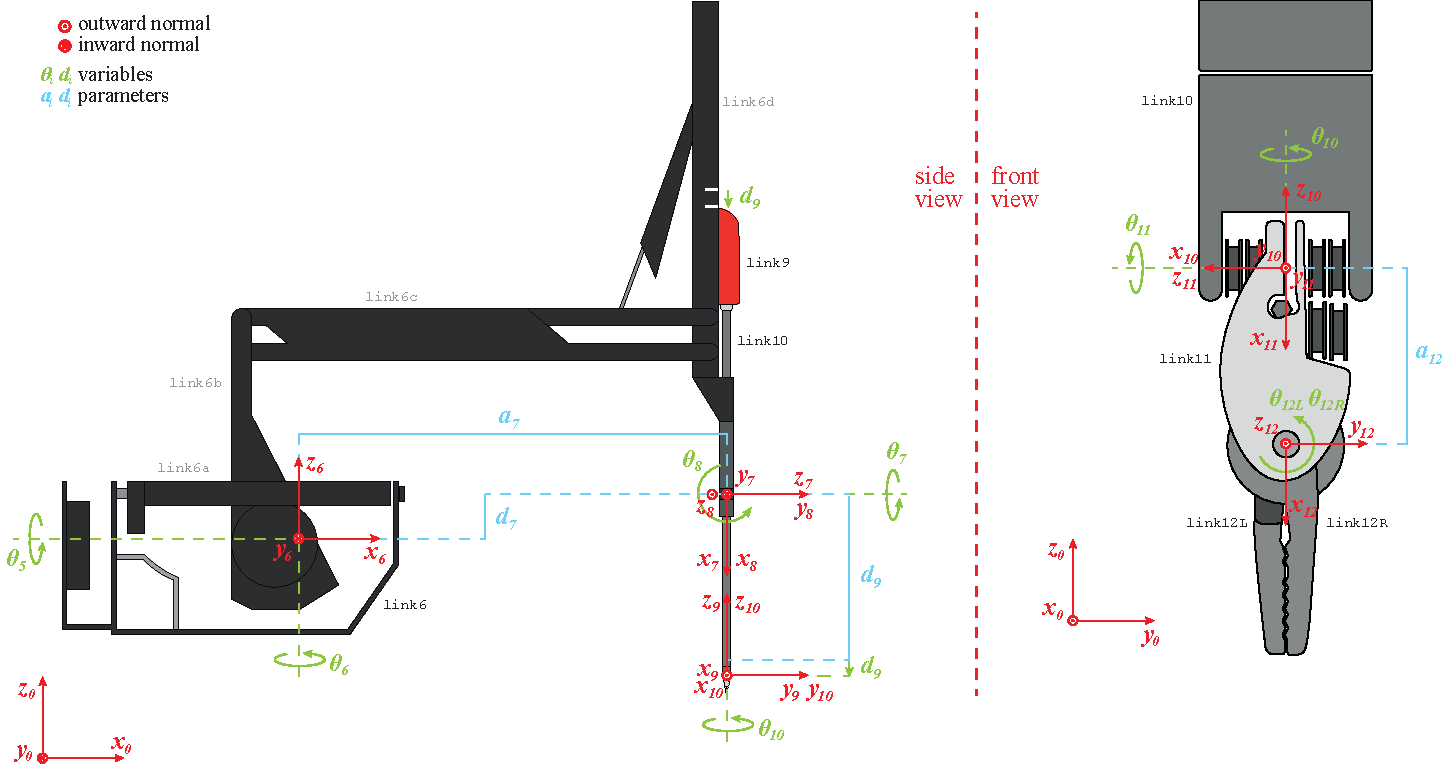
\includegraphics[width=1.15\textwidth]{p4_hand_compromise_frames_chapter.pdf}\label{fig:p4_hand_compromise_frames_chapter}}%
	\caption{Orientation and position of coordinate frames $\Psi_7$, $\Psi_8$, etc. corresponding to the controllable joints of the robotic patient manipulator.  For convenience of placing the hand roll and pitch frames in the pivot point in the new kinematic description in \autoref{fig:p4_hand_compromise_frames_chapter}, a virtual link is inserted in the \texttt{xacro} file after each of these two joints.}
	\label{fig:robot_hand_kinematics}
\end{figure}


For more details on the old and new kinematic descriptions implemented in \gls{ros}; including all measurements of parameters, gearing ratios, code for testing the kinematic description in Matlab, and measurements of distances for different configurations; please refer to \autoref{sec:existing_kinematics} and \ref{sec:app_activejoints_kinematics} in \autoref{app:kinematic_model_robot}.










\subsection{Employing Inverse Kinematics for a Controller in 3D Cartesian Space}
The controller is developed for 3D position and orientation control of the tool tip, and relies on the \gls{kdl} inverse kinematics solver to map from the desired 3D Cartesian space configuration to a prudent 6D joint space position of the da Vinci robotic patient manipulator, in order to pass the transformed joint position commands to the low level controllers (see \autoref{fig:overview}).

The \gls{ik} \gls{kdl} solver employed in \gls{ros} relies on the kinematic chain from the URDF, which is generated from the \texttt{xacro} link and joint kinematic description as presented in %\autoref{app:kinematic_model_robot}, the model implemented in ROS defined in
\autoref{sec:app_activejoints_kinematics}. From this chain (\texttt{my\_chain} in the below example) a \gls{fk} position solver is created along with an \gls{ik} velocity solver in order to define the \gls{ik} position solver:

\begin{lstlisting}[language=xml]
//Create solver based on kinematic chain
KDL::ChainFkSolverPos_recursive fksolver(my_chain);
KDL::ChainIkSolverVel_pinv iksolverv(my_chain);
KDL::ChainIkSolverPos_NR iksolver = KDL::ChainIkSolverPos_NR(my_chain,fksolver,iksolverv,100,1e-6);

KDL::JntArray q(my_chain.getNrOfJoints());
KDL::JntArray q_init(my_chain.getNrOfJoints());

//Set destination frame
double x, y, z;
std::cout << "Set end-effector position <x y z>:" << std::endl;
std::cin >> x >> y >> z;
KDL::Vector dest_pos(x,y,z);
KDL::Frame dest_frame(dest_pos);

// Compute!
int ret = iksolver.CartToJnt(q_init,dest_frame,q);
\end{lstlisting}

The \gls{kdl} \gls{ik} position solver uses the Newton-Raphson iterative numerical technique through the function \texttt{CartToJnt} to determine a prudent joint configuration implementing the desired Cartesian configuration (given as \texttt{dest\_frame} in the above example). In the above example the initial guess \texttt{q\_init} of the joint configuration is the current joint configuration, and hence care should be taken to only command small changes in configuration for the sake of fast convergence of the \gls{ik} solution.


Three dimensional positions of the tool tip is described in a frame oriented as the inertial frame and offset such that a robot configuration with all free angles and slide set to zero equals a position of the tool tip in [0,0,0].
The ellipsoid enclosing the region $\mathcal{X}_u$ in \autoref{fig:robot_hand_unsafe_region} is defined as the zero level set of a function of the form:
\begin{equation}
B(x,y,z) = -\left(  \left(\frac{x-c_x}{r_x}\right)^2 + \left(\frac{y-c_y}{r_y}\right)^2 + \left(\frac{z-c_z}{r_z}\right)^2 - 1 \right)
\end{equation}
\begin{tabular}{rl}
where&\\
$[c_x\,\, c_y\,\, c_z]$ & is the coordinate of the center of the ellipsoid\\
$[r_x\,\, r_y\,\, r_z]$ & is the length of the semi-axes of the ellipsoid\\
\end{tabular}


\section{Modelling of Robot Hand Movement}
\textcolor{red}{Make measurement of step for cases: x-axis, y-axis, z-axis, and xyz at the same time.}

\section{Safe Controller Design for First Order System}

A decoupled first order system is assumed for each of the three axes on the form

\begin{equation}
\small
\dot{\begin{bmatrix}
	x\\y\\z
	\end{bmatrix}} =
\begin{bmatrix}
-1/\tau & 0 & 0\\0 & -1/\tau & 0 \\ 0 & 0 & -1/\tau
\end{bmatrix}
\begin{bmatrix}
x\\y\\z
\end{bmatrix} +
\begin{bmatrix}
1/\tau& 0 & 0 \\ 0& 1/\tau & 0 \\0& 0& 1/\tau
\end{bmatrix} 
\left(
\begin{bmatrix}
\bar{N} & 0 & 0 \\0 & \bar{N} & 0 \\0& 0& \bar{N}
\end{bmatrix}
\begin{bmatrix}
x_{ref}\\y_{ref}\\z_{ref}
\end{bmatrix}
-
\begin{bmatrix}
k_x & 0 & 0 \\0 & k_y & 0 \\0& 0&  k_z
\end{bmatrix}
\begin{bmatrix}
x\\y\\z
\end{bmatrix}
\right)
\end{equation}

\textcolor{green}{Giver modellen mening?}

THIS IS ONLY POSITION, NOT ORIENTATION

\section{Safe Controller Design for Second Order System}